\documentclass[11pt]{article}

\usepackage[margin=1in]{geometry}
\usepackage[T1]{fontenc}
\usepackage[utf8]{inputenc}
\usepackage{lmodern}
\usepackage{microtype}
\usepackage{amsmath,amssymb}
\usepackage{booktabs}
\usepackage{graphicx}
\usepackage{xcolor}
\usepackage[colorlinks=true, linkcolor=blue!60!black, citecolor=blue!60!black,
            urlcolor=blue!60!black]{hyperref}
\usepackage[numbers]{natbib}

\newcommand{\gap}{\textsc{gap}}

\title{Watching Without Seeing Time:\\
A Per-Question-Type Ablation of Modality Usage\\ in a Video--Language Model}
\author{Marcos Lahoz\\
\small Universit\'e Paris-Saclay\\
\small \texttt{marcoslahozy14@gmail.com}}
\date{June 2026}

\begin{document}
\maketitle

\begin{abstract}
Multiple-choice VideoQA accuracy is routinely read as evidence that a model
\emph{understands video}. We measure what a modern open video--language model
actually uses when it answers. Using a small model-agnostic ablation harness
(\texttt{vmd}), we evaluate Qwen2.5-VL-3B on a balanced 240-question subset of
NExT-QA under controlled evidence conditions: full frames, no frames (blind),
temporally shuffled frames (order destroyed, content preserved), and dropped
frames (content destroyed). Three results follow. (i)~The language prior is
large: blind accuracy is $0.433$ against a $0.20$ chance level. (ii)~The value
of the video is concentrated in \emph{descriptive} questions ($+0.344$ over
blind) and \emph{causal} questions ($+0.200$); on \emph{temporal} questions ---
the category that nominally requires watching the video --- frames add only
$+0.033$. (iii)~Temporal order is never used: fully shuffling the frame
sequence does not reduce accuracy in any question group, while dropping 75\% of
the frames costs at most $0.04$. On this benchmark slice the model behaves as a
\emph{bag-of-frames} system, consistent with single-frame biases reported for
earlier video--language architectures. The harness, per-item predictions and a
one-click reproduction notebook are public.
\end{abstract}

\section{Introduction}

Benchmark accuracy is an aggregate that can hide how a prediction is produced.
In multimodal question answering, a model can score well by exploiting
regularities of the question--answer text alone, without using the
media~\citep{goyal2017vqa}. For video, the failure has a second, subtler level:
a model may genuinely use the \emph{content} of the frames while remaining
indifferent to their \emph{order} --- behaving as an image model applied to a
bag of frames~\citep{buch2022revisiting,lei2023revealing}.

This note asks a narrow, answerable question: \emph{when Qwen2.5-VL-3B answers
NExT-QA questions, which part of the video signal is it actually using?} We
decompose the question along two axes that are usually conflated:

\begin{enumerate}
  \item \textbf{Presence}: does accuracy drop when the frames are removed
        entirely (the \emph{collapse gap} between full and blind accuracy)?
  \item \textbf{Structure}: does accuracy drop when the frames are kept but
        their temporal order is destroyed (shuffle), versus when their content
        is destroyed (drop)?
\end{enumerate}

\noindent and we resolve both per NExT-QA question type (causal, temporal,
descriptive), since the categories make different demands on temporal
understanding by construction~\citep{xiao2021nextqa}.

\section{Method}

\paragraph{Harness.} \texttt{vmd}~\citep{lahoz2026vmd} treats the model as a
black box behind a one-method interface: \texttt{answer(item, view)}, where the
\emph{view} controls which evidence channels the model may see and at what
corruption severity. The experiment grid is therefore a property of the
harness, not of the model: full evidence, blind (no media), and graded
corruption of a single channel. All metrics derive from per-item correctness
records, which we release alongside the code.

\paragraph{Frame-level conditions.} Eight frames are sampled uniformly from
each clip (resized to $\leq 448$\,px on the longest side). The two corruption
operators are chosen to dissociate order from content:
\emph{shuffle}$(s)$ permutes a fraction $s$ of the sampled frames --- the frame
multiset is unchanged, only temporal structure is lost; \emph{drop}$(s)$
removes a fraction $s$ of the frames --- content is genuinely lost. A model
that reasons over temporal structure must degrade under full shuffle; a model
that only aggregates per-frame evidence will degrade under drop but not under
shuffle.

\paragraph{Model and prompting.} Qwen2.5-VL-3B-Instruct~\citep{bai2025qwen25vl}
with greedy decoding. The prompt presents the frames (when available), the
question and the five options, and requests the option index; unparseable
outputs fall back to the first option (deterministic; they are rare).

\section{Experimental setup}

From the NExT-QA multiple-choice test split (8{,}564 questions) we sample 240
questions balanced over the eight fine-grained types (30 each), grouped as
causal (CW, CH; $n{=}60$), temporal (TN, TC, TP; $n{=}90$) and descriptive (DC,
DL, DO; $n{=}90$).\footnote{Annotations and videos from the
\texttt{lmms-lab/NExTQA} distribution; the subset-building script
(\texttt{scripts/prepare\_nextqa.py}) is seeded and extracts only the required
clips.} Six conditions are evaluated: full, blind, shuffle at
$s\in\{0.5, 1.0\}$ and drop at $s\in\{0.5, 0.75\}$ --- $1{,}440$ inference
calls in total, no training. Chance accuracy is $0.20$.

\section{Results}

\begin{table}[t]
\centering
\caption{Accuracy of Qwen2.5-VL-3B on the balanced NExT-QA subset
($n{=}240$, 8 frames) under controlled evidence conditions.}
\label{tab:overall}
\begin{tabular}{lc}
\toprule
Condition & Accuracy \\
\midrule
Full (8 frames)            & 0.625 \\
Blind (no frames)          & 0.433 \\
\textbf{Collapse gap}      & \textbf{0.192} \\
\midrule
Shuffle 50\% of frames     & 0.625 \\
Shuffle 100\% of frames    & 0.650 \\
Drop 50\% of frames        & 0.592 \\
Drop 75\% of frames        & 0.600 \\
\bottomrule
\end{tabular}
\end{table}

\begin{table}[t]
\centering
\caption{Per-question-group breakdown. $\Delta$ columns are relative to the
full condition of the same group.}
\label{tab:groups}
\setlength{\tabcolsep}{5pt}
\begin{tabular}{lrccccccc}
\toprule
Group & $n$ & Full & Blind & \gap{} & Shuf.\,100\% & $\Delta$\,shuf. & Drop\,75\% & $\Delta$\,drop \\
\midrule
Causal      & 60 & 0.600 & 0.400 & $+0.200$ & 0.650 & $+0.050$ & 0.567 & $-0.033$ \\
Temporal    & 90 & 0.511 & 0.478 & $\mathbf{+0.033}$ & 0.533 & $+0.022$ & 0.511 & $\phantom{-}0.000$ \\
Descriptive & 90 & 0.756 & 0.411 & $+0.344$ & 0.767 & $+0.011$ & 0.711 & $-0.044$ \\
\bottomrule
\end{tabular}
\end{table}

\begin{figure}[t]
  \centering
  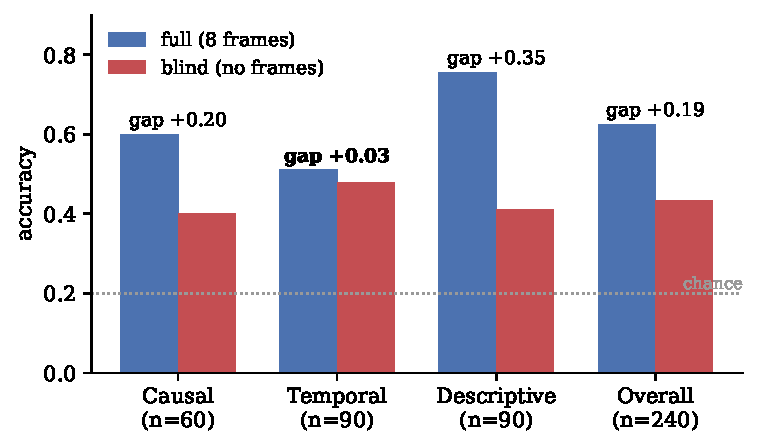
\includegraphics[width=0.78\linewidth]{figures/gap_by_group.pdf}
  \caption{Full vs.\ blind accuracy per question group. The collapse gap ---
  what the video actually buys --- is large for descriptive questions, moderate
  for causal ones, and nearly zero for temporal ones.}
  \label{fig:gap}
\end{figure}

\begin{figure}[t]
  \centering
  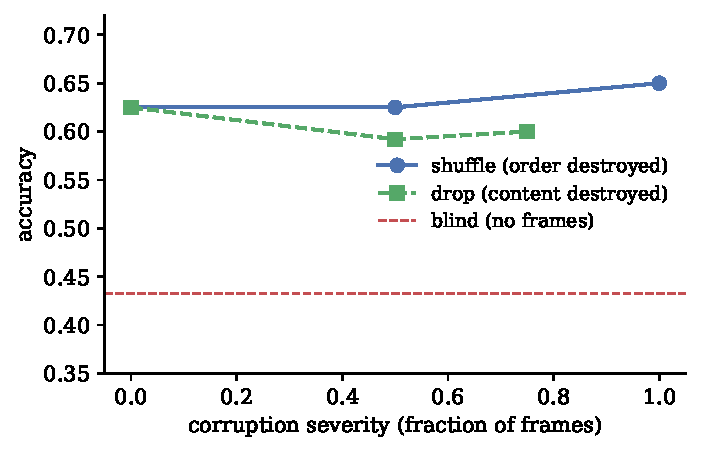
\includegraphics[width=0.62\linewidth]{figures/corruption_curves.pdf}
  \caption{Accuracy under graded frame corruption (overall, $n{=}240$).
  Destroying temporal order (shuffle) has no effect; destroying content (drop)
  produces a modest decline. Neither approaches the blind baseline.}
  \label{fig:curves}
\end{figure}

\paragraph{The language prior is large.} Blind accuracy is $0.433$
(Table~\ref{tab:overall}), more than twice the chance level. Nearly half of
this benchmark slice is answerable from the question--option text alone, in
line with prior-exploitation findings in image VQA~\citep{goyal2017vqa}. Any
headline VideoQA score on such data overstates video understanding by roughly
this margin.

\paragraph{The video helps where it is least needed.} The collapse gap is
$+0.344$ on descriptive questions and $+0.200$ on causal ones, but only
$+0.033$ on temporal questions (Table~\ref{tab:groups},
Figure~\ref{fig:gap}). On the category whose answers are \emph{defined} by
temporal relations --- before/after, order of events --- the model is barely
better with the video than without it. Its temporal accuracy ($0.511$) is also
the lowest of the three groups despite temporal blind accuracy being the
\emph{highest} ($0.478$): the questions are not harder as text; the model
simply extracts almost nothing temporal from the frames.

\paragraph{Order is never used; little content suffices.} Fully shuffling the
frame order leaves accuracy unchanged in every group ($\Delta$ between $+0.01$
and $+0.05$, within sampling noise; Figure~\ref{fig:curves}), so no measurable
part of the model's behaviour depends on temporal structure --- including on
temporal questions. Dropping 75\% of the frames (8\,$\to$\,2) costs at most
$0.044$: the per-frame evidence the model does use is highly redundant. Both
observations match the \emph{bag-of-frames} picture: per-frame perception
aggregated order-insensitively, as reported for earlier video--language models
via atemporal probes~\citep{buch2022revisiting} and single-frame
training~\citep{lei2023revealing}, and consistent with the compositional
temporal-reasoning gaps exposed by AGQA~\citep{grunde2021agqa}. Our
contribution is to isolate the same bias in a modern open VLM with a single
unified ablation grid, resolved per question type, at the cost of
$\sim$1{,}400 inference calls and no training.

\section{Limitations}

$n{=}240$ gives roughly $\pm 0.06$ binomial standard error per group, so small
$\Delta$s are not individually significant --- the conclusions rest on the
\emph{pattern} (a near-zero temporal gap that is consistent across shuffle and
drop probes), not on any single cell. Results are for one model (3B), one
frame budget (8), one decoding scheme, and one benchmark; the natural next
experiment is the same grid at 7B/72B to test whether scale buys temporal
usage, and at 16--32 frames to rule out under-sampling as the cause of the
temporal gap. Multiple-choice answer parsing, while deterministic, can
interact with option phrasing. NExT-QA inherits its videos from VidOR;
findings may not transfer to longer or denser footage.

\section{Reproducibility}

Code, the seeded subset builder, the executed notebook, per-item prediction
records for every condition (\texttt{records\_video.json}) and this report are
available at \url{https://github.com/mlahozy21/video-modality-diagnostics}.
The full experiment is inference-only and runs on a single L4 GPU in under an
hour.

\bibliographystyle{plainnat}
\bibliography{references}

\end{document}
